\documentclass[11pt]{article}
\usepackage[margin=1in]{geometry}
\usepackage{titlesec}
\usepackage{url}
\usepackage{hyperref}
\usepackage{amsmath}
\usepackage{enumitem} % in preamble
\usepackage{graphicx}
\graphicspath{{../Screenshots/}}


\begin{document}
\setcounter{section}{5}
\section{Preliminary Calculations and Feasibility Tests}
Two solutions are to be compared in order to determine the best choice for a constricting mechanism: 
\begin{enumerate}
    \item Hexagonal Diaphragm
    \item Needle Valve
\end{enumerate}
The \textbf{required relationship} of $D_{\text{eff}} = A_1(T-T_{\text{ref}})+A_0$ is linear. It is therefore advantageous 
to keep a linear relationship in the mechanism's parameters. The following calculations will determine feasibility of both solutions to linearly set an effective diameter "$D_{\text{eff}}$". 
\subsection{Determine linearity of Hexagonal Diaphragm(solution 1)}
\subsubsection{Determine linear relationship of hexagonal side length and  $D_{\text{eff}}$:}
let the area of a hexagon be \boldmath{$A_{hex}$} and its side length be \boldmath{$s$}.
\begin{align}
    D_{\text{eff}} &= \sqrt{\frac{4A}{\pi}}
    \\
    A_{\text{hex}} &= \frac{4\sqrt{3}}{2}s^2
\end{align}
eq (1) $\circ$ eq(2):
\\~\\
    $D_{\text{eff}} = \sqrt{\frac{4A_{\text{hex}}}{\pi}} = \sqrt{\frac{8}{pi}}\sqrt[4]{3}s
    $
    \\
 let $k = \sqrt{\frac{8}{pi}}\sqrt[4]{3}$
    \\
    \boldmath{$D_{\text{eff}} = ks $}: Clear proof that the effective diameter of a hexagonal geometry is linearly proportional to its side length s.
\subsubsection{Determine if linear actuation(input) corresponds to linear change in side length s(output):}
Let change in input (displacement) be $\Delta a$, and the output (a change in the side length of the hexagonal opening) be $\Delta s$.
\begin{center}
    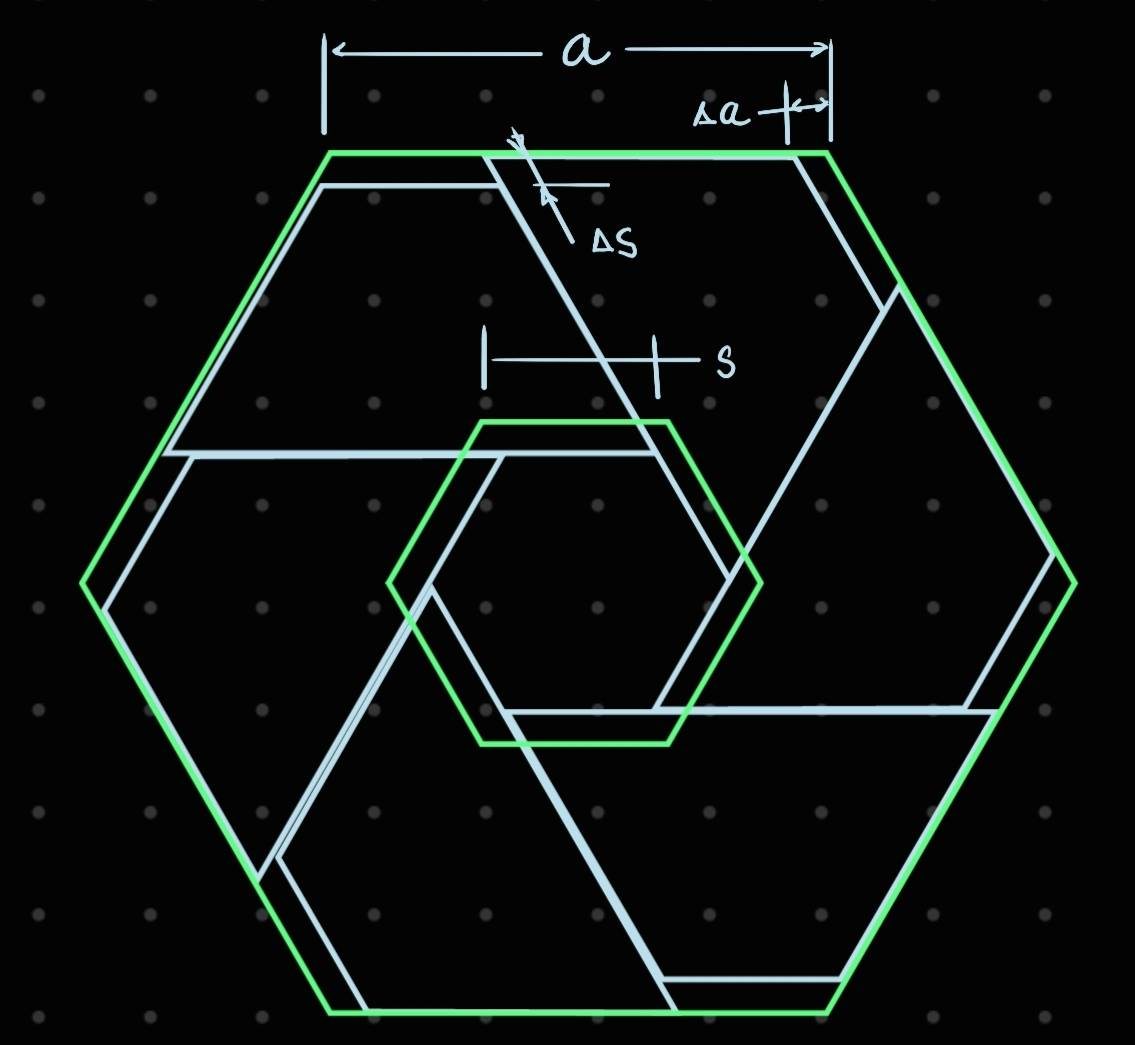
\includegraphics[width=150pt]{hexagongeometry.jpg}
    \hspace{1em}
    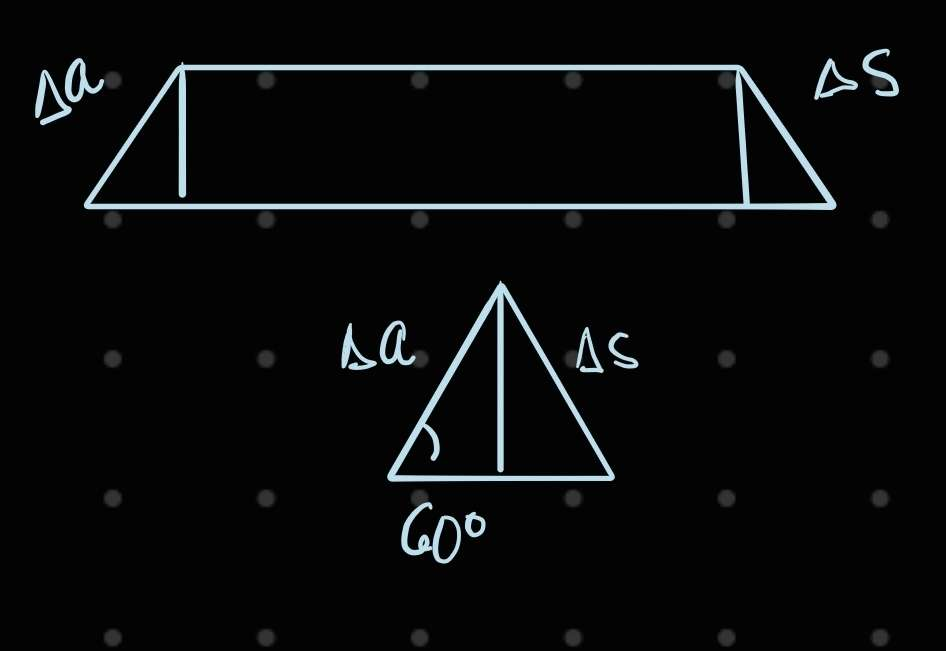
\includegraphics[width=150pt]{equilateraltriangle.jpg}
\end{center}
Looking at both diagrams, it is geometrically apparent that $\Delta s$ and $\Delta a$ are two sides in the same equilateral triangle, thus they are not only linearly related, they are also equivalent (slope of 1).
\newpage
\subsection{Determine linearity of Needle Valve(solution 2)}

\newpage
\subsection{Error propagation}
Tolerance is one of the main requirements given the scale of the device. This means error propagation must be considered.
\\~\\
From the required relationship and tolerances: 
\begin{align*}
    D_{\text{eff}} &= A_1(T-T_{\text{ref}})+A_0
    \\
    A_1 &= -6\cdot10^{-5}\pm 5\%
    \\
    A_0 &= 0.01 \pm 5\%
\end{align*}
This gives us uncertainty values of:
\begin{align*}
    u_{A_1} &= A_1 \cdot 0.05 = -3 \cdot 10^{-6}
    \\
    u_{A_0} &= A_0 \cdot 0.05 = 5 \cdot 10^{-4}
    \\
    \theta_{A_1} &= \frac{\delta D}{\delta A_1} = \Delta T
    \\
    \theta_{A_0} &= \frac{\delta D}{\delta A_0} = 1
\end{align*}
\subsubsection{Calculating uncertainty of $D_{eff}$:}
\begin{align*}
    u_{D} &= \sqrt{(\theta u)_{A_1}^2+(\theta u)_{A_0}^2}
    \\
    &= \sqrt{-9\cdot10^{-12}\Delta T^2 + 2.5\cdot10^{-7}}
\end{align*}
At this point, we have all the terms to assemble the maximum and minimum bounds of $D_{eff}$ given the design conditions $\Delta T$.
$$D_{eff}(\Delta T_{\text{min}}) = 0.0151\pm 0.00043$$
$$D_{eff}(\Delta T_{\text{max}}) = 0.0067\pm 0.00047$$
\newpage
\subsection{Conclusion}
The calculations performed determined if a solution behaves linearly with an input. This linear behavior is important because the required relationship of $D_{\text{eff}} = A_1(T-T_{\text{ref}})+A_0$ is linear with respect to the temperature change.
\\~\\
Solutions considered:
\begin{enumerate}
    \item The Hexagonal Diaphragm has a clear linear relationship with an actuator input proven by the results:
    \begin{enumerate}
        \item from section 6.1.1: $D_{\text{eff}} = ks $
        \item from section 6.1.2: $\Delta s = \Delta a$
    \end{enumerate}
    \item The Needle Valve does not readily accomodate a linear temperature-diameter relationship as required and must include custom-made geometry before it can be used.
\end{enumerate}
Therefore, the Hexagonal Diaphragm is a better solution than the Needle Valve since it can effectively accomodate the linear temperature-diameter relationship of $D_{\text{eff}} = A_1(T-T_{\text{ref}})+A_0$.
\end{document}